\section*{Front-End Web Development with React}

This course provide an introduction to the React framework, its components and some basic elements like routing, forms and animations. Shared state management, with the corresponding tools like Redux, is another important topic covered alongside fetching data.

\subsection*{React Overview}

React is a JavaScript library for building component-based user interfaces using a declarative approach. React focuses only on user interface and is designed for speed, simplicity and scalability.

A React component is a JavaScript class or function that  is imported from the React Module. It is then rendered using the React's rendering function \texttt{ReactCOM.render(...)}.

\subsubsection*{Components}
A component is an indipendent and reusable set of React elements that should appear on screen. Every component can accepts any input and is composed of React tags, that always start with a capital letter, and native tags, which start with lowercase letters and are treated as DOM tags.
Every component has a local state which can hold multiple information that can be passed to children components using \texttt{props}. The state is an immutable object that can be updated using the \texttt{setState(...)} directive. This function accept the property to update and merge it with the actual state. Only class components can have a local state. The state must never be manipulated directly.

Handling event is possible in a similar way as on DOM elements:

\begin{figure}[h]
    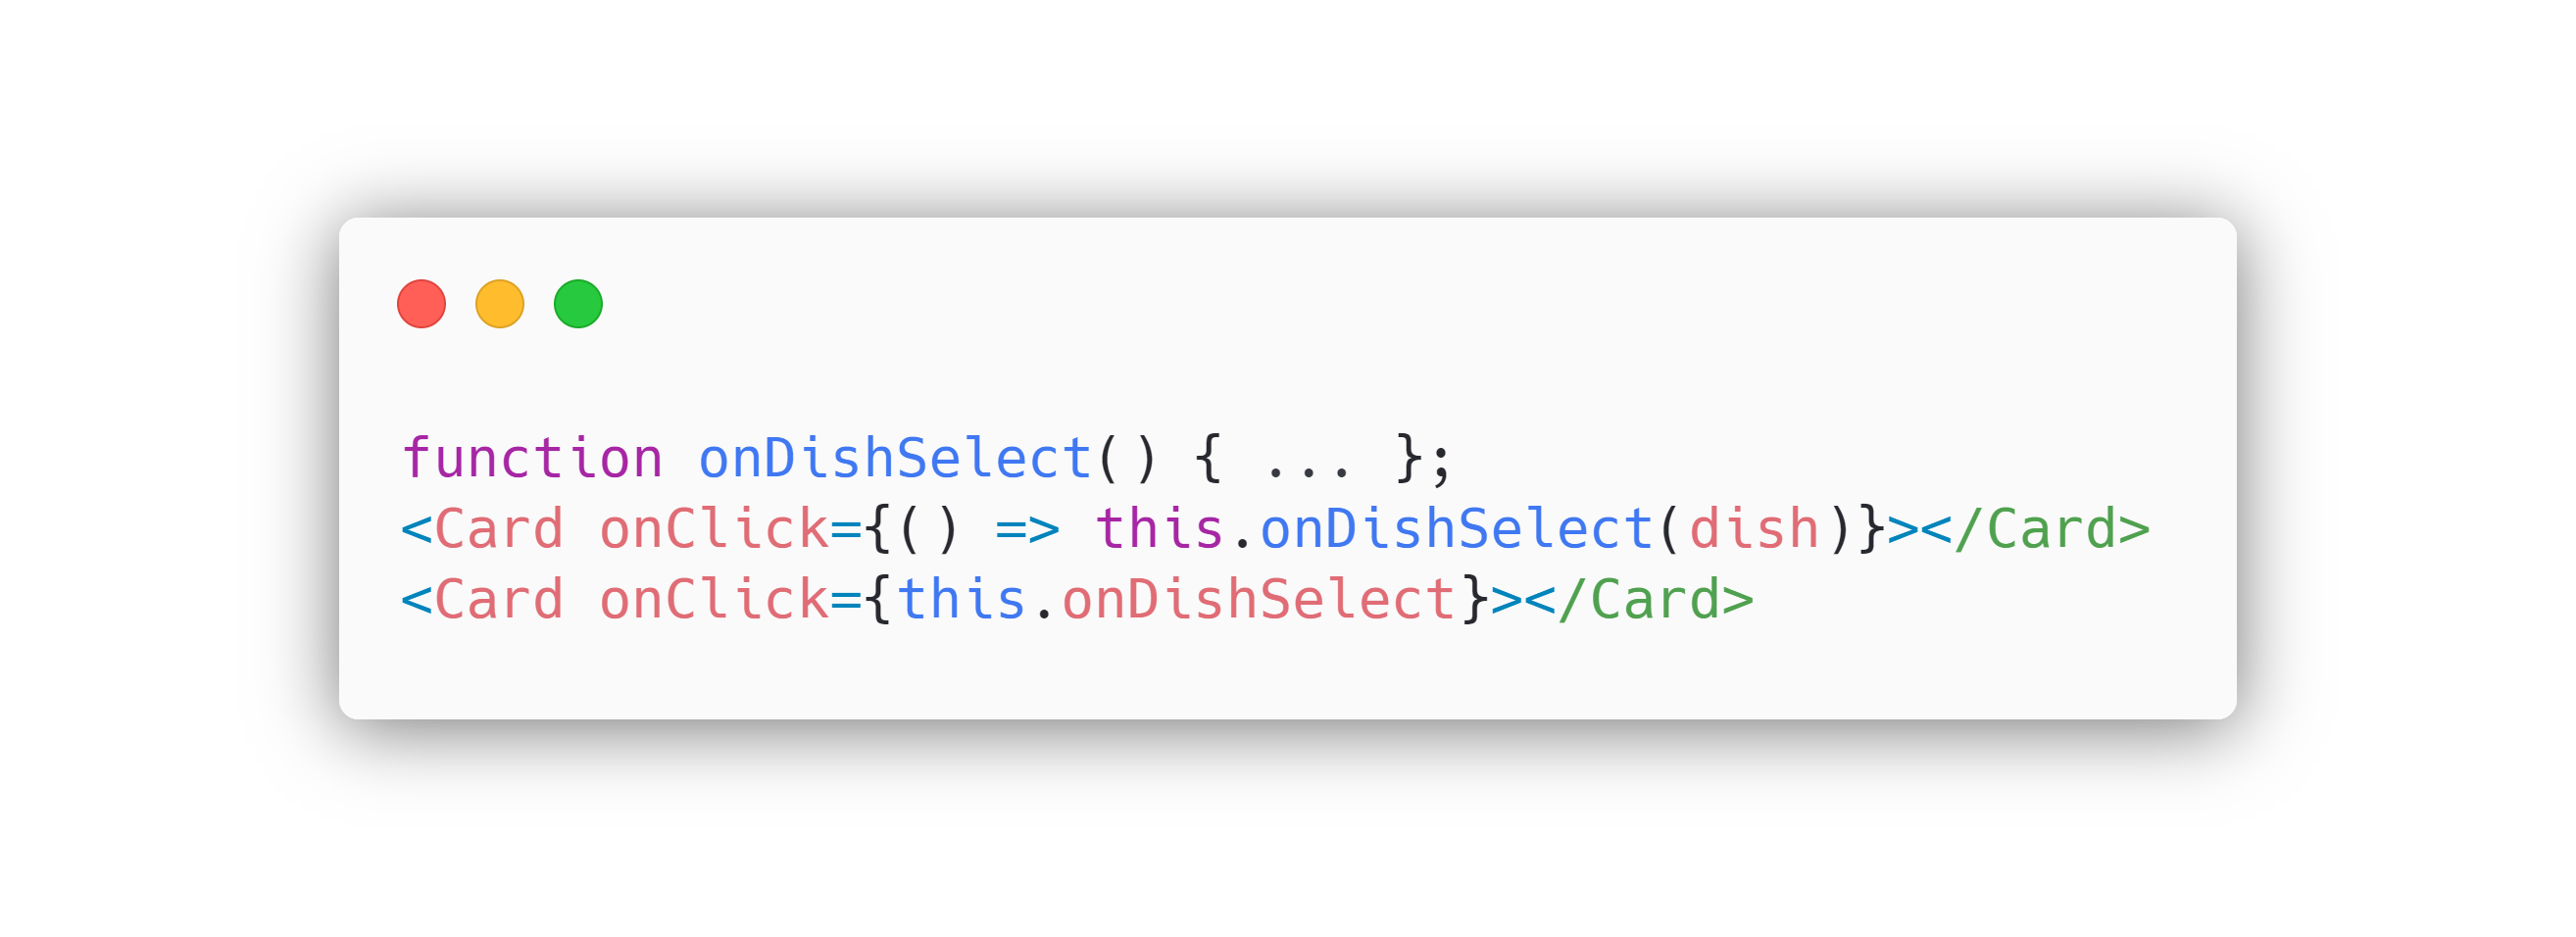
\includegraphics[width=\textwidth]{assets/react-event-handling.png}
    \caption{Event handling when clicking on div}
    \label{fig:event-handling}
\end{figure}

In Figure \ref{fig:event-handling} is possible to see how map a function to a click event on the React element \texttt{Card}.

\paragraph*{Lifecycle}
React provides life cycle hooks/methods that can be invoked to perform certain operations. Component is created and then mounted in the application and when it's not required anymore is unmounted. There are three stages of lifecycle: mounting, updating and unmounting. Each stage provide, when component is declared as class, several methods like a construcor (mounting), \texttt{componentDidMount()} (called after mounting is finished), \texttt{render()} (call when rendering UI) and many others.

\paragraph*{Functonal vs Class}
Until the release of \texttt{React 16.8} in 2018 there were two ways of declaring a component: class component or functional component. Functional components are s JavaScript function that returns a React element, can receive props but cannot provide local state or lifecycle hooks. 
\begin{figure}
    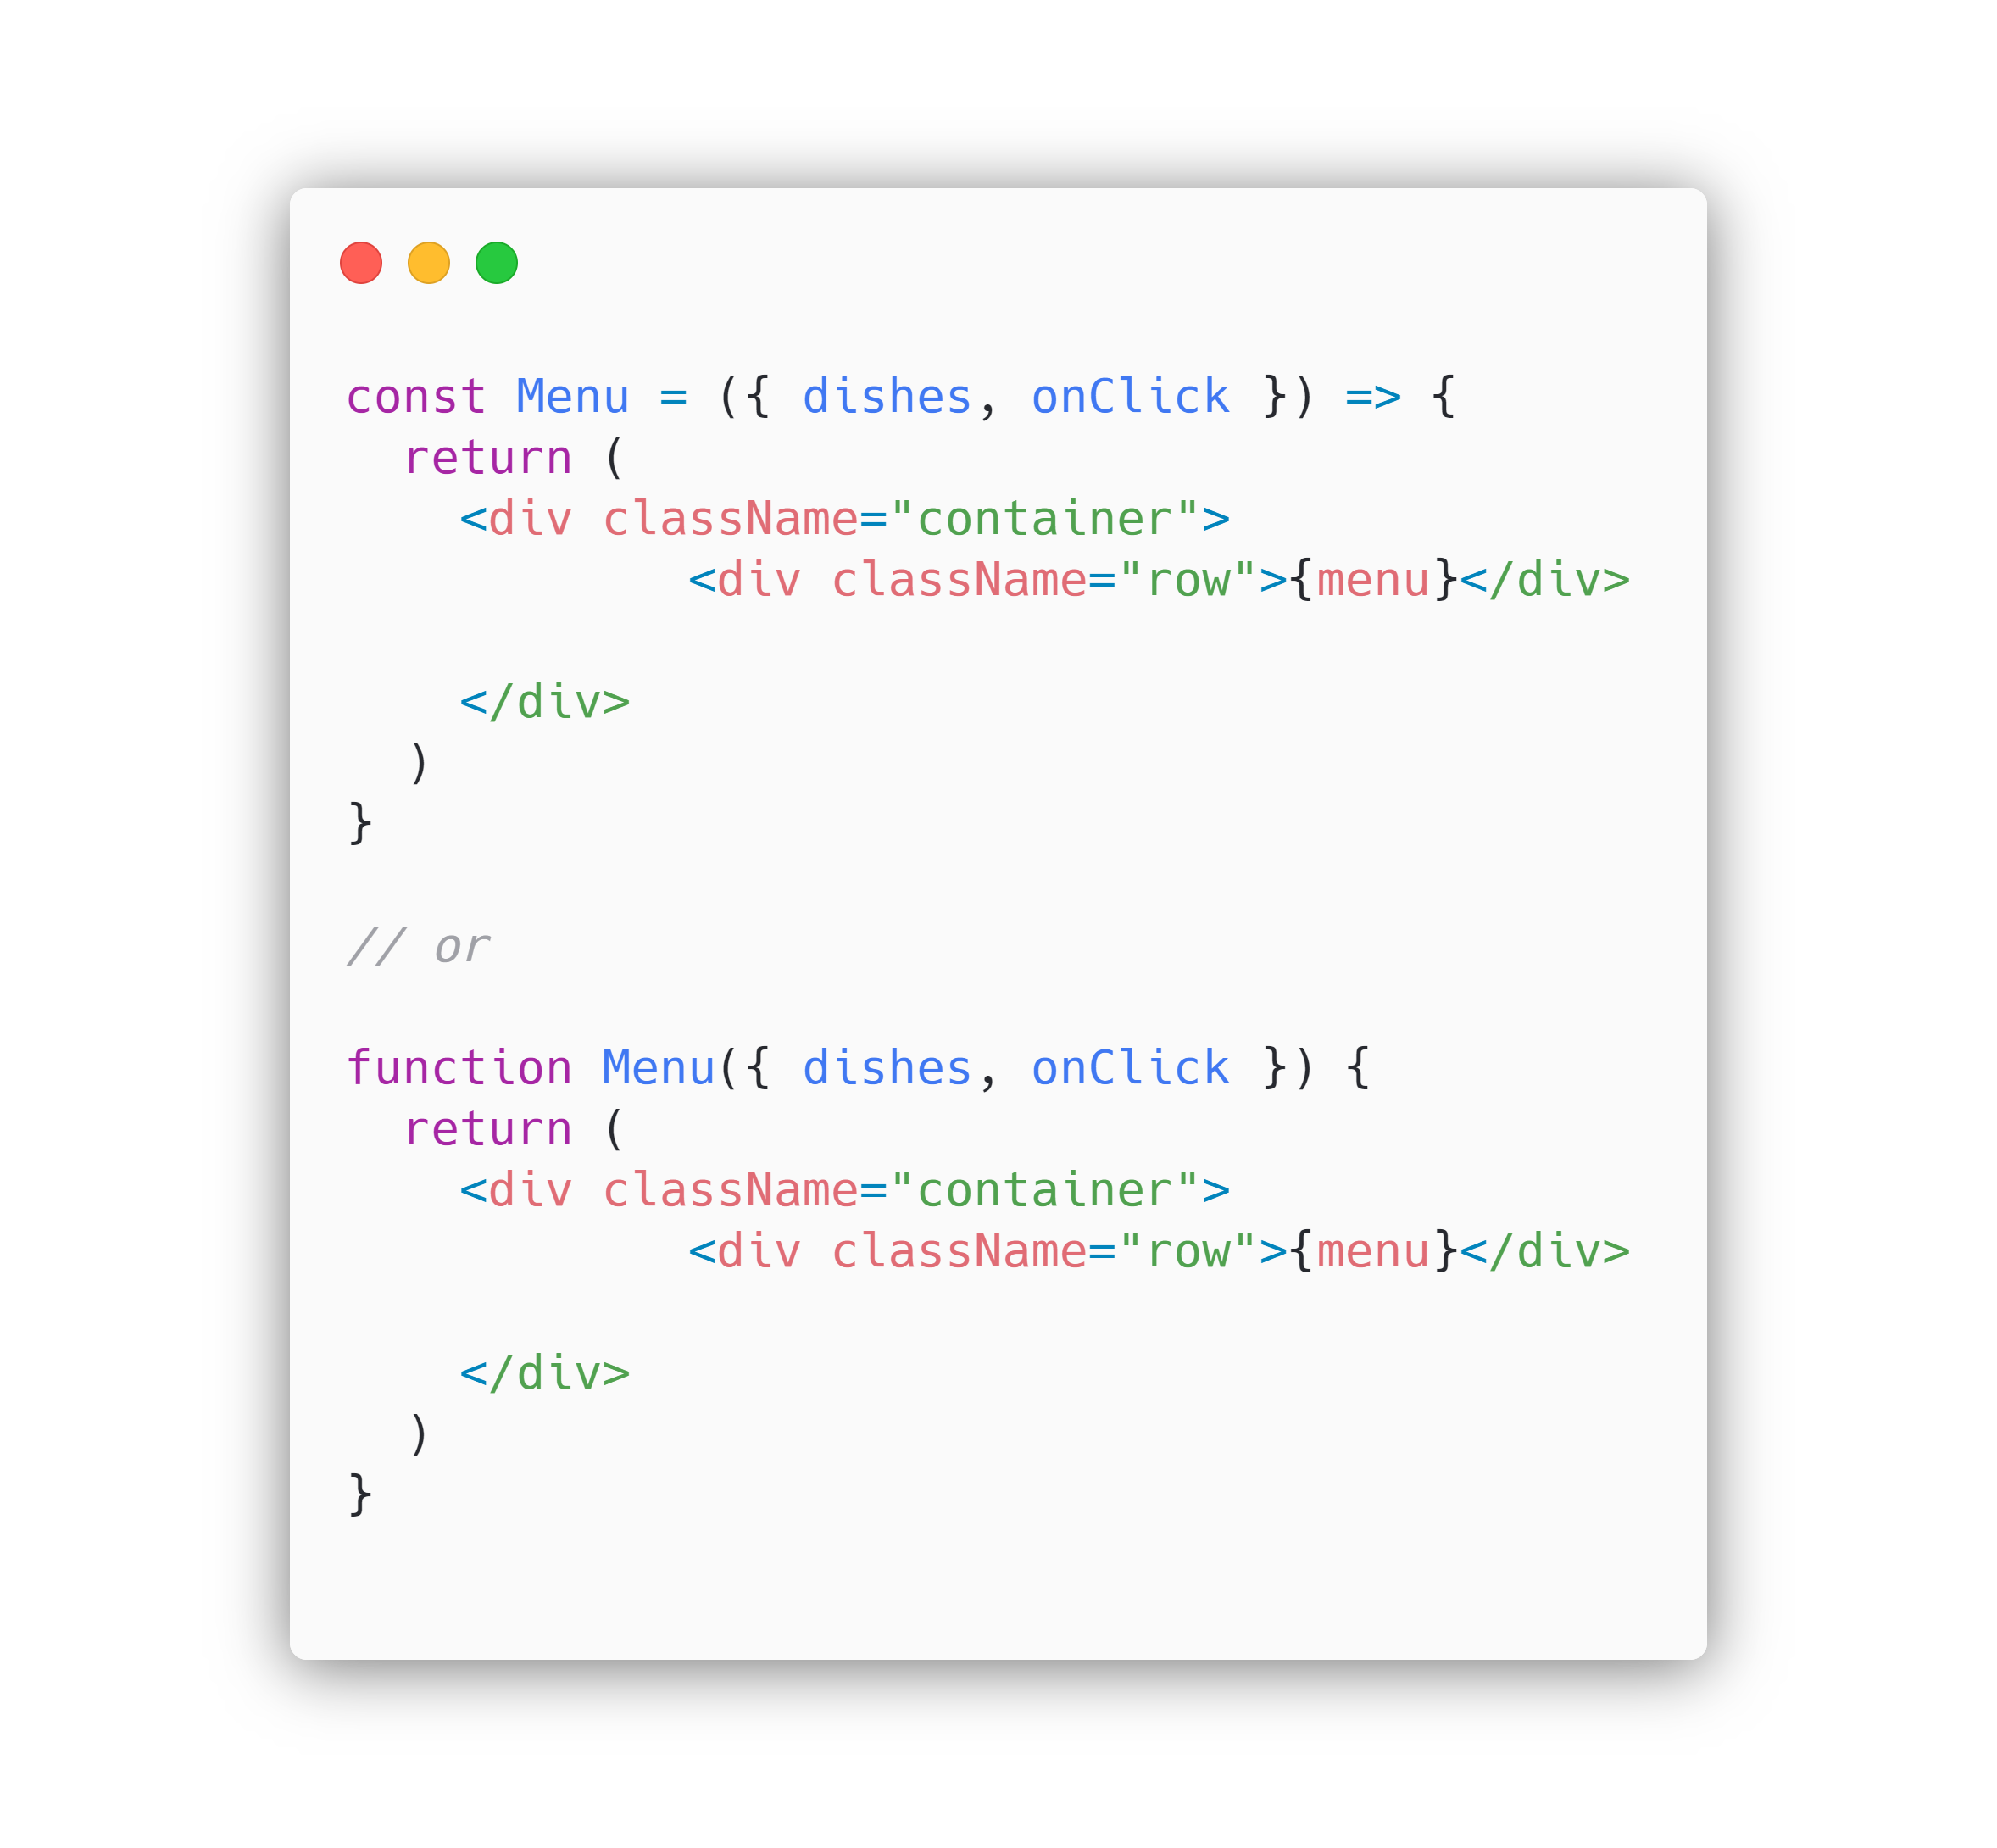
\includegraphics[width=\textwidth]{assets/class-vs-functional.png}
    \caption{Ways to define a functional components as function or arrow function}
\end{figure}

In React 16.8 it was introduced React Hooks to use lifecycle hooks also in functional component. This topic is not covered in courses, but will be discussed in the appendix of this document.

\paragraph*{Document Object Model}
In the browser there is an object called \texttt{Browser DOM} (Document Object Model) and is the representation of the structure and data of a webpage. React uses a lightweight version of DOM called \texttt{Virtual DOM}, which uses an in-memory tree data structure of plain JavaScript objects, is extremely fast to manipulate compared to browser DOM and is fully recreated on every setState. 

There is a diffing algorithm that detect which nodes are changed and updates the only the minimum number of components in the sub-tree that is updated.

\subsubsection*{React Router}
React Router gives the ability to navigate between views using links. It's a module that need to be additionally installed into the React application called \texttt{react-router-dom}. It is a collection of navigational components that enable navigation among views and support a browser-based bookmarkable URLs to navigate in the web app. It is also possible to pass optional parameters.
